\section{Introduction}
\label{sec:intro}

Curriculum learning (CL) proposed by~\citet{bengio2009curriculum} provides performance improvements on a number of machine learning tasks.
It mimics the learning process of humans by training models with samples in a 
more meaningful order, i.e., from the easy ones to the hard ones.
Therefore, ranking training samples by difficulty lies in the core of CL, 
which is also the key challenge when it's applied to natural language generation (NLG) 
tasks.

Previous work on CL for NLG focuses on measuring the difficulty of training samples 
in two ways. One is to resort to human-crafted rules based on various linguistic features 
and human observations~\cite{liu2018curriculum,kocmi2017curriculum}. 
The other uses models either trained from outside data or the same data but
in previous epochs/steps~\cite{zhou2020uncertainty,kumar2019reinforcement,shen2020cdl}.
Either way seeks to produce a numeric score for each training sample relying on domain expertise so that it can
be ranked,  
%More importantly, both approaches relied on domain expertise to design
%features to be used in the rules or models, 
making it difficult to generalize 
to different tasks. For example, summarization focuses more on generating concise 
outputs while style transfer emphasizes style changes. So the former should pay 
attention to the ratio between the lengths of the output and the input (the more compressed
the more difficult), while the 
latter should focus on differences in style between the input and output (the more
different the more difficult).
Designing a comprehensive or universal scoring function is difficult or 
even impossible under this definition of CL.
%\citet{xu2020curriculum} proposed training classifiers
%-based approaches. 
%For example, \cite{shen2020cdl} trained independent emotion classifier and use accuracy to reorder training samples. Other works~\cite{zhou2020uncertainty,kumar2019reinforcement} utilized models trained in the previous epoch/step for ranking. 
%In a word, these approaches are highly relied on expertise and lack of generalization ability among different tasks.
\begin{figure*}[th]
	\centering
	\begin{minipage}[t]{0.33\linewidth}
		\centering
		\subfloat[Sample-wise Curriculum Learning]{
			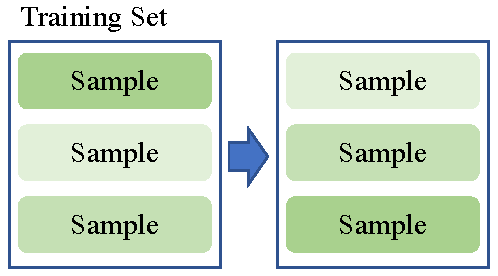
\includegraphics[scale=0.55]{cl.pdf}
			%\caption{fig1}
		}%
	\end{minipage}%
	\begin{minipage}[t]{0.33\linewidth}
		\centering
		\subfloat[Token-wise ``Curriculum Learning'']{
			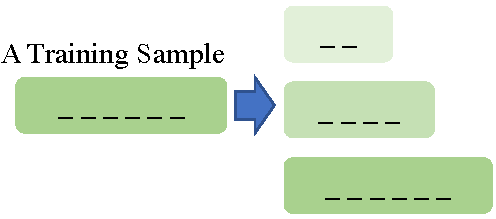
\includegraphics[scale=0.5]{daicl.pdf}
			%\caption{fig2}
		}%
	\end{minipage}%
	\begin{minipage}[t]{0.33\linewidth}
		\centering
		\subfloat[In-sample Curriculum Learning]{
			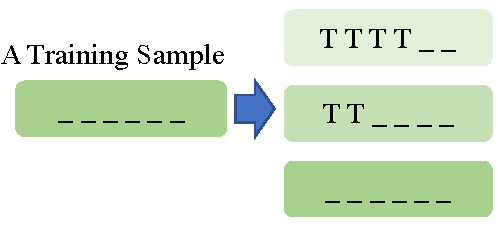
\includegraphics[scale=0.5]{icl.pdf}
			%\caption{fig2}
		}%
	\end{minipage}%
	\centering
	\caption{Illustrations of the main ideas of traditional sample-wise CL, Liang et al.~\shortcite{liang-etal-2021-token-wise}'s TCL and our ICL. 
Green box refers to samples in different difficulty levels. The darker, the harder. ``T'' refers to a known token while ``\_'' refer to a token to be
generated in the output sequence of a sample during training.}
	\label{fig:intro}
\end{figure*}


%An alternative approach is to looking down 

In this paper, we propose an alternative to sample-wise CL, which we call 
in-sample CL (ICL). 
ICL re-orders the learning sequence within the sample. 
One particular ICL re-ordering strategy which we find effective is to predict the 
last few tokens given a long prefix first from the original output, and then gradually increase the tokens
at the end while shortening the prefix, to create an easy-to-hard training
order. Such a curriculum learning strategy focuses more on the difficulty of language generation itself,
leading to a better generalization ability among tasks.

Actually, we are not the first to propose the idea of ICL.
\citet{liang-etal-2021-token-wise} introduced the notion of ``token-wise curriculum
learning(TCL)''. %for machine translation. 
Illustrations of TCL, ICL and the traditional CL are shown in \figref{fig:intro}.
At a first glance,
their idea is similar to ours, except they consider generating the first few tokens
in the output sequence to be easier than generating a longer sequence in the output. 
However, the real difference is that while we consider each training sample in full
length, only with variable-length prefixes, they create training samples of increasing
output length by cutting the sentences short. %(also see \figref{fig:intro}). 
Even though they also have a ``soft'' version of the approach, the essence of TCL
is still augmenting data
with incomplete and even
``incorrect'' training samples. %, which is not really curriculum 
%learning in the classic sense. 
%but rather imperfect data augmentation especially under the ``hard'' setting.
Therefore, in our opinion, \citeauthor{liang-etal-2021-token-wise}'s work is not really curriculum learning in the classic sense, but rather imperfect data augmentation, especially under their ``hard'' setting.
%This means that they are essentially augmenting data from the original
%training pair, only to produce \textit{incorrect} training samples because the output
%sequences are cut short. 
This also explains why it doesn't work as well as our method in a range of generation tasks 
including reading comprehension,
dialogue summarization, style transfer, question generation and 
news summarization. 
%In our experiments, we also show that our approach can be
%combined with other sample-wise CL approaches to achieve better results.

%Reconsidering the NLG tasks, neural models under the encoder-decoder architecture are trained to predict the output given the input through maximum likelihood estimation, no matter how long the output is.
%However, predicting the whole output sequence is tough at the start of training iterations reflected by poor results. If more information about the output is given, the generation task will be easier

%Reconsidering the NLG tasks, neural models under the encoder-decoder architecture have achieved a remarkable success. 
%These models are trained to predict the output given the input through maximum likelihood estimation, no matter how long the output is.
%However, predicting the whole output sequence is tough at the start of training iterations reflected by poor results.
%
%Inspired by the idea of training from easy to difficult, we avoid the requirement of ranking training samples in traditional curriculum learning and newly propose to do \textbf{in-sample curriculum learning(ICL)}. The model is trained to complete the end of output first and gradually learns to generate the whole output sequence.
%According to this intuition, we introduce the proportional ICL strategy that manipulating a percentage to determine the prediction length for each sample during training.
%We did experiments on a number of generation tasks including  reading comprehension, dialogue summarization, style transfer, question generation and news summarization. Comprehensive experiments and analysis show the favorable of our approach over the strong baselines. 
In a word, our contributions are:
\begin{itemize}
	\item As far as we know, we are the first to propose the real in-sample curriculum learning
for text generation (\secref{sec:icl}).
	\item We propose a novel ICL learning algorithm (\secref{sec:iclalgorithm}). 
Together with our sequence completion ICL curriculum, it achieves significant improvements over 
the strong baselines on different NLG tasks, demonstrating strong generalization ability
(\secref{sec:experiment}).
	\item The ICL can be combined with other traditional CL for further performance gains 
(Section~\ref{sec:tracl}). 
\end{itemize}

